% Options for packages loaded elsewhere
\PassOptionsToPackage{unicode}{hyperref}
\PassOptionsToPackage{hyphens}{url}
%
\documentclass[
]{book}
\usepackage{amsmath,amssymb}
\usepackage{lmodern}
\usepackage{ifxetex,ifluatex}
\ifnum 0\ifxetex 1\fi\ifluatex 1\fi=0 % if pdftex
  \usepackage[T1]{fontenc}
  \usepackage[utf8]{inputenc}
  \usepackage{textcomp} % provide euro and other symbols
\else % if luatex or xetex
  \usepackage{unicode-math}
  \defaultfontfeatures{Scale=MatchLowercase}
  \defaultfontfeatures[\rmfamily]{Ligatures=TeX,Scale=1}
\fi
% Use upquote if available, for straight quotes in verbatim environments
\IfFileExists{upquote.sty}{\usepackage{upquote}}{}
\IfFileExists{microtype.sty}{% use microtype if available
  \usepackage[]{microtype}
  \UseMicrotypeSet[protrusion]{basicmath} % disable protrusion for tt fonts
}{}
\makeatletter
\@ifundefined{KOMAClassName}{% if non-KOMA class
  \IfFileExists{parskip.sty}{%
    \usepackage{parskip}
  }{% else
    \setlength{\parindent}{0pt}
    \setlength{\parskip}{6pt plus 2pt minus 1pt}}
}{% if KOMA class
  \KOMAoptions{parskip=half}}
\makeatother
\usepackage{xcolor}
\IfFileExists{xurl.sty}{\usepackage{xurl}}{} % add URL line breaks if available
\IfFileExists{bookmark.sty}{\usepackage{bookmark}}{\usepackage{hyperref}}
\hypersetup{
  pdftitle={EFI Task Views},
  pdfauthor={Ecological Forecasting Initative},
  hidelinks,
  pdfcreator={LaTeX via pandoc}}
\urlstyle{same} % disable monospaced font for URLs
\usepackage{longtable,booktabs,array}
\usepackage{calc} % for calculating minipage widths
% Correct order of tables after \paragraph or \subparagraph
\usepackage{etoolbox}
\makeatletter
\patchcmd\longtable{\par}{\if@noskipsec\mbox{}\fi\par}{}{}
\makeatother
% Allow footnotes in longtable head/foot
\IfFileExists{footnotehyper.sty}{\usepackage{footnotehyper}}{\usepackage{footnote}}
\makesavenoteenv{longtable}
\usepackage{graphicx}
\makeatletter
\def\maxwidth{\ifdim\Gin@nat@width>\linewidth\linewidth\else\Gin@nat@width\fi}
\def\maxheight{\ifdim\Gin@nat@height>\textheight\textheight\else\Gin@nat@height\fi}
\makeatother
% Scale images if necessary, so that they will not overflow the page
% margins by default, and it is still possible to overwrite the defaults
% using explicit options in \includegraphics[width, height, ...]{}
\setkeys{Gin}{width=\maxwidth,height=\maxheight,keepaspectratio}
% Set default figure placement to htbp
\makeatletter
\def\fps@figure{htbp}
\makeatother
\setlength{\emergencystretch}{3em} % prevent overfull lines
\providecommand{\tightlist}{%
  \setlength{\itemsep}{0pt}\setlength{\parskip}{0pt}}
\setcounter{secnumdepth}{5}
\usepackage{booktabs}
\usepackage{titling}
\pretitle{\begin{center} 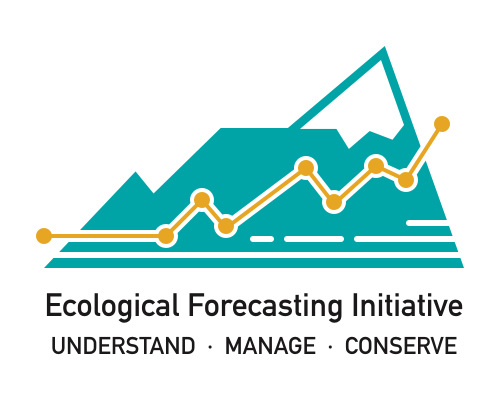
\includegraphics[width=2in,height=2in]{images/EFI_Logo-1.jpg}\LARGE\\}
\posttitle{\end{center}}
\ifluatex
  \usepackage{selnolig}  % disable illegal ligatures
\fi
\usepackage[]{natbib}
\bibliographystyle{apalike}

\title{EFI Task Views}
\author{Ecological Forecasting Initative}
\date{Last modified: 2021-06-24}

\begin{document}
\maketitle

{
\setcounter{tocdepth}{1}
\tableofcontents
}
\hypertarget{introduction}{%
\chapter*{Introduction}\label{introduction}}
\addcontentsline{toc}{chapter}{Introduction}

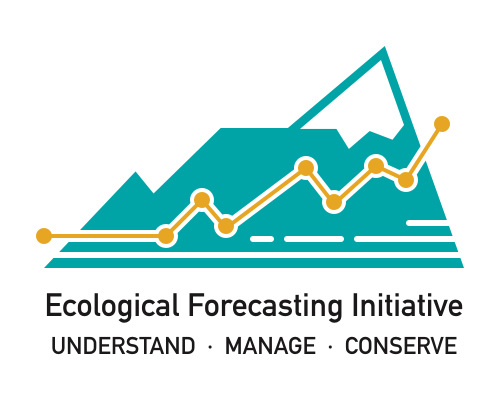
\includegraphics[width=0.25\textwidth,height=\textheight]{images/EFI_Logo-1.jpg}

The EFI \href{https://ecoforecast.org/methods-tools/}{Methods} and \href{https://ecoforecast.org/cyberinfrastructure/}{Cyberinfrastructure} EFI Working Groups are compiling common tasks in ecological forecasting and methods and tools to help with tasks commonly used in ecological forecasting for the following categories.

\begin{itemize}
\tightlist
\item
  Reproducible Forecasting Workflows
\item
  Modeling \& Statistical resources, including Uncertainty Quantification \& Propagation
\item
  Data Ingest, Cleaning, and Management
\item
  Visualization, Decision Support, and User Interfaces.
\end{itemize}

These Resources and tools listed in the four categories of tasks are meant to be living documents. This list is not meant to be a comprehensive overview of all possible resources, as there are some tasks where there are hundreds of different tools available. Instead we focus on commonly used tools. However, if there are often used tools and resources we are missing, we welcome input from anyone --- suggestions can be shared as Issues to the \href{https://github.com/eco4cast/taskviews}{eco4cast/taskview GitHub repository}.

\hypertarget{reproducible-forecasting-workflows}{%
\chapter{Reproducible Forecasting Workflows}\label{reproducible-forecasting-workflows}}

Text from the \href{https://ecoforecast.org/reproducible-forecasting-workflows/}{Reproducible Workflow EFI page} will be transferred here

\hypertarget{uncertainty-quantification-data-assimilation-modeling-statistics}{%
\chapter{Uncertainty quantification, Data assimilation, Modeling \& Statistics}\label{uncertainty-quantification-data-assimilation-modeling-statistics}}

\hypertarget{overview}{%
\section{Overview}\label{overview}}

Curators: Abby Lewis\textsuperscript{1}, Ben Toh\textsuperscript{2}, Jake Zwart\textsuperscript{3}, Alexey Shiklomanov\textsuperscript{4}, Leah Johnson\textsuperscript{1}, Ethan White\textsuperscript{2}, Hassan Moustahfid\textsuperscript{5}, Kelly Heilman\textsuperscript{6}, Ash Griffin\textsuperscript{7}, Jody Peters\textsuperscript{8}, Quinn Thomas\textsuperscript{1}, Mike Dietze\textsuperscript{9}

\emph{\textsuperscript{1}Virginia Tech, \textsuperscript{2}University of Florida, \textsuperscript{3}USGS, \textsuperscript{4}NASA, \textsuperscript{5}NOAA, \textsuperscript{6}University of Arizona, \textsuperscript{7}MailChimp, \textsuperscript{8}University of Notre Dame, \textsuperscript{9}Boston University}

The crux of a successful forecasting system is an effective model with properly specified uncertainty. Numerous techniques are available to create a model for a given forecasting problem, and each modeling technique will require different mechanisms for incorporating, quantifying, and propagating uncertainty. Here, we outline the tools available for both empirical (statistical, Bayesian, and machine learning) and mechanistic models (Figure 1: C). To expand on existing modeling resources, we then describe how uncertainty can be incorporated into a forecasting workflow using different types of model and tools for assimilating new data to update a forecast (Figure 1: D).

\begin{figure}
\centering
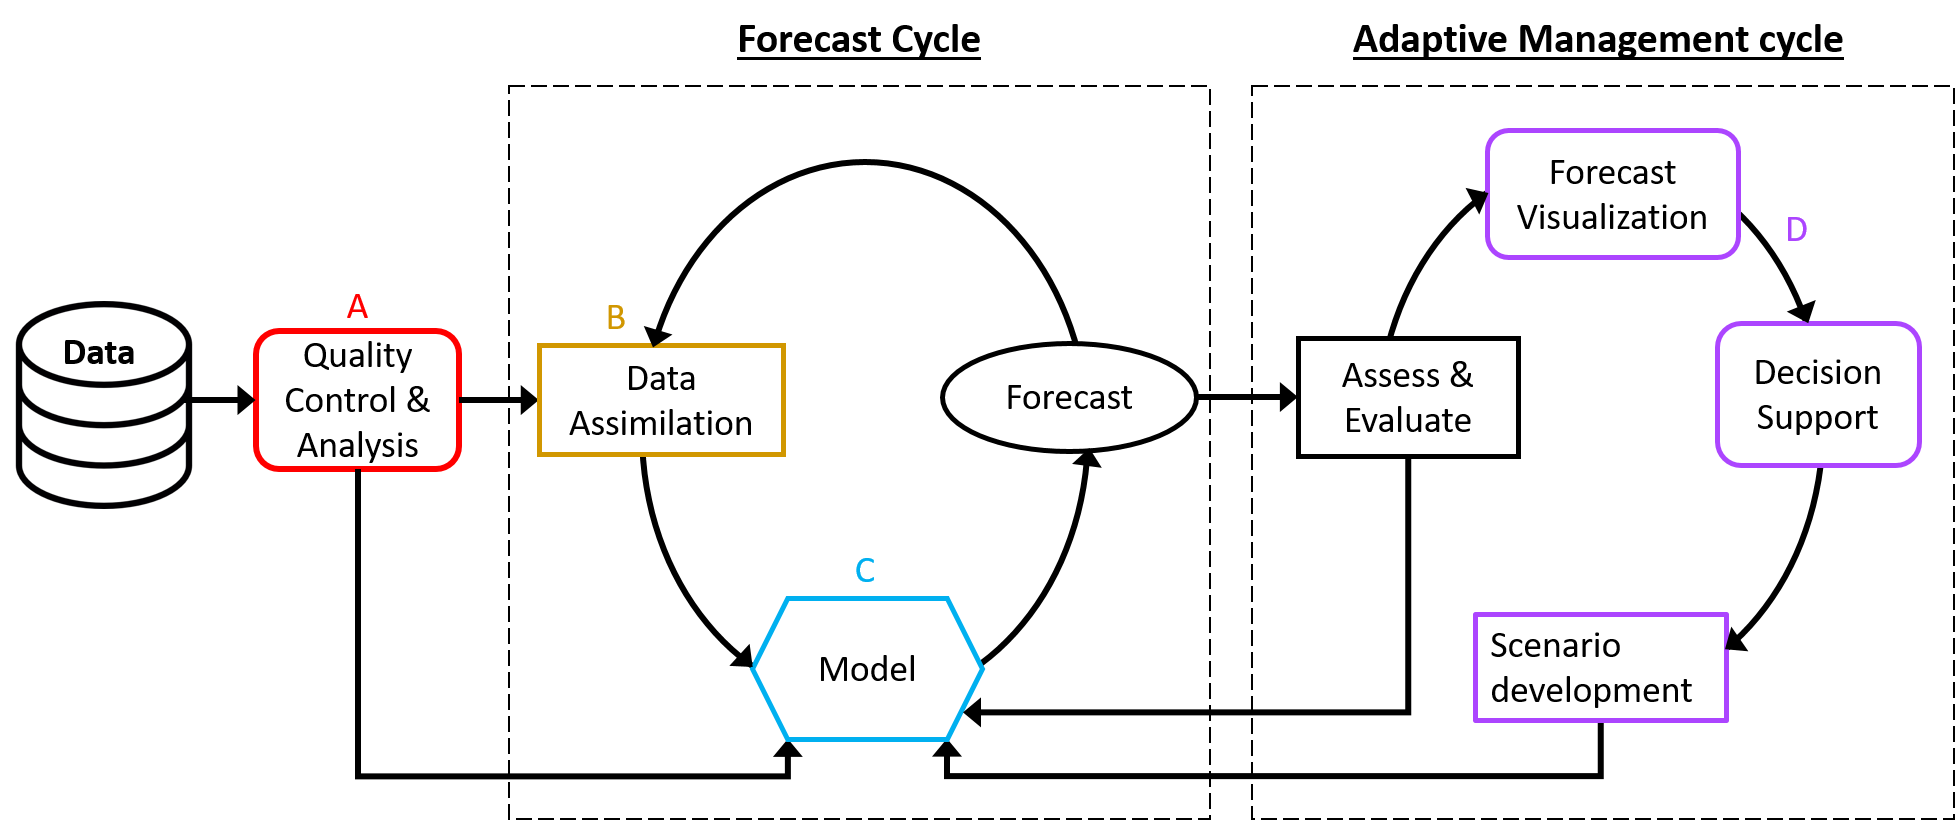
\includegraphics{images/Fig1_StatsMethodsUncertaintyTaskView.png}
\caption{Figure 1. Conceptual diagram of the components in the forecast workflow, including the iterative forecast and adaptive management cycles. A (Data Ingest, Cleaning, Management) and D (Visualization/Decision Support Tools, User Interface) will be described in future task views. B (Data Assimilation) and C (Model) are described below.}
\end{figure}

\hypertarget{empirical-models}{%
\section{Empirical models}\label{empirical-models}}

In general, empirical models let data speak for itself, making inferences and predictions without extensively encoding the underlying ecological process. These models are often fast and computationally efficient when making predictions. However, they are only informed by previous values in the dataset and therefore may be unlikely to perform well outside of the range of observed conditions. Furthermore, improper variable selection and assumptions on distributions can cause inaccurate predictions. In this section, we outline tools for two categories of empirical models: statistical models and machine learning.

\hypertarget{statistical-model-frequentist}{%
\subsection{Statistical model (frequentist)}\label{statistical-model-frequentist}}

Statistical models use historical data to estimate statistical parameters, then use those estimates to forecast into the future. In this section we focus on some of the more commonly used tools for fitting statistical models and making forecasts within a frequentist framework. Time series models, e.g.~Auto Regressive Integrated Moving Average (\href{https://en.wikipedia.org/wiki/Autoregressive_integrated_moving_average}{ARIMA}) models, are a common choice of statistical model relevant to forecasting. These models focus on learning the temporal pattern of the past, including seasonality and temporal autocorrelation, and project this pattern into the future in a forecasting setting.

\hypertarget{tools-for-frequentist-models}{%
\subsubsection{Tools for frequentist models}\label{tools-for-frequentist-models}}

The following are commonly used tools for fitting and running frequentist models for the interpreted programming languages R and Python. See the \href{https://ecoforecast.org/reproducible-forecasting-workflows/\#scripted}{Reproducible Forecasting Workflows post} for more details on these two interpreted languages.

\begin{itemize}
\tightlist
\item
  \textbf{R}

  \begin{itemize}
  \tightlist
  \item
    The \href{https://stat.ethz.ch/R-manual/R-devel/library/stats/html/00Index.html}{stats} (aka ``base R'') package provides time series functions such as \href{https://stat.ethz.ch/R-manual/R-devel/library/stats/html/ts.html}{ts()} and \href{https://stat.ethz.ch/R-manual/R-devel/library/stats/html/arima0.html}{arima()} for representing time series objects and fitting ARIMA models.\\
  \item
    The \href{https://cran.r-project.org/web/packages/forecast/index.html}{forecast package} offers more useful tools for fitting ARIMA models. For example, \href{https://www.rdocumentation.org/packages/forecast/versions/8.14/topics/auto.arima}{auto.arima()} finds the best set of parameters for both seasonal and non-seasonal components of the ARIMA model based on Akaike information criterion (AIC) or Bayesian information criterion (BIC); \href{https://www.rdocumentation.org/packages/forecast/versions/8.14/topics/forecast}{forecast()} makes predictions and great forecasting plots (with prediction uncertainty!) based on your choice of ARIMA model. It also provides useful statistical tests and cross-validation functions. See \href{https://otexts.com/fpp2/arima.html}{this online textbook}.\\
  \item
    The \href{https://cran.r-project.org/web/packages/nlme/index.html}{nlme}, \href{https://cran.r-project.org/web/packages/glmmTMB/index.html}{lme4} and \href{https://cran.r-project.org/web/packages/glmmTMB/index.html}{glmmTMB} packages can be used to fit Generalized Linear Mixed Models (GLMM), incorporating autoregressive model (AR1) structure alongside other random effects.
  \item
    The \href{https://cran.r-project.org/web/packages/mgcv/index.html}{mgcv} and \href{https://cran.r-project.org/web/packages/gamm4/index.html}{gamm4} packages provide the \href{https://www.rdocumentation.org/packages/mgcv/versions/1.8-35/topics/gamm}{gamm()} function to fit Generalized Additive Mixed Models, incorporating AR1 structure, random effects and splines, and spatial smoothers.
  \end{itemize}
\item
  \textbf{Python}

  \begin{itemize}
  \tightlist
  \item
    The \href{https://www.statsmodels.org/stable/index.html}{statsmodels} module provides the core functions for working with ARIMA models including \href{https://www.statsmodels.org/stable/generated/statsmodels.tsa.arima.model.ARIMA.html\#statsmodels.tsa.arima.model.ARIMA}{arima.model.ARIMA()} for fitting models of specific orders and functions for comparing the fits of models with different orders.\\
  \item
    The \href{https://pypi.org/project/pmdarima/}{pmdarima} module provides a high level wrapper to statsmodels with equivalent functionality to `forecast::auto.arima()' in R. The \href{https://alkaline-ml.com/pmdarima/modules/generated/pmdarima.arima.auto_arima.html?highlight=auto_arima}{auto\_arima()} function provides automated model selection to determine the best seasonal and non-seasonal ARIMA models based on a suite of information criteria. This package also provides useful statistical tests and cross-validation functions.
  \end{itemize}
\end{itemize}

\hypertarget{statistical-model-bayesian}{%
\subsection{Statistical model (Bayesian)}\label{statistical-model-bayesian}}

In a Bayesian framework, all fitted parameters have a probability distribution. This is useful as it enables robust accounting of parameter uncertainty, and allows for the model to be informed by existing data or expertise. Often, a Bayesian framework also allows the user to fit more complicated and hierarchical time series models, while accounting for uncertainty in parameters, drivers, and observation data. Options for fitting Bayesian models include

\begin{enumerate}
\def\labelenumi{\arabic{enumi}.}
\tightlist
\item
  working directly with Markov chain Monte Carlo (MCMC) samplers,
\item
  interfacing with existing MCMC or Gibbs samplers such as Just Another Gibbs Sampler (JAGS), Bayesian inference Using Gibbs Sampling (BUGS), or Stan,
\item
  using readily available ``native'' functions, and
\item
  Laplace approximation.
  These methods are all described in more detail below.
\end{enumerate}

\hypertarget{work-directly-with-markov-chain-monte-carlo-mcmc}{%
\subsubsection{Work directly with Markov chain Monte Carlo (MCMC)}\label{work-directly-with-markov-chain-monte-carlo-mcmc}}

\begin{itemize}
\tightlist
\item
  \textbf{R}

  \begin{itemize}
  \tightlist
  \item
    The \href{https://cran.r-project.org/web/packages/mcmc/index.html}{mcmc} package facilitates sampling from a posterior distribution using the Metropolis algorithm and provides other useful helper functions\\
  \item
    The \href{https://cran.r-project.org/web/packages/MCMCpack/index.html}{MCMCpack} package also provides a function to sample from a distribution using the Metropolis algorithm and provides other useful helper functions\\
  \item
    The \href{https://cran.r-project.org/web/packages/BayesianTools/index.html}{BayesianTools} package provides functions to run a range of different MCMC algorithms as well as non-MCMC sampling algorithms such as rejection sampling and sequential Monte Carlo (SMC). Also provides model selections and multi-model inference functionality. Treats the model as a `black box' so particularly handy for calibrating mechanistic models.
  \end{itemize}
\item
  \textbf{Python}

  \begin{itemize}
  \tightlist
  \item
    The \href{https://docs.pymc.io/}{pymc3} module allows models to be written using the Python language, and fits the model using various sampling algorithms.
  \end{itemize}
\end{itemize}

\hypertarget{interface-with-jagsbugsstan}{%
\subsubsection{Interface with JAGS/BUGS/Stan}\label{interface-with-jagsbugsstan}}

Instead of working directly with MCMC samplers, a model can be specified in the \href{https://mcmc-jags.sourceforge.io/}{JAGS} (Just Another Gibbs Sampler), \href{https://www.mrc-bsu.cam.ac.uk/software/bugs/}{BUGS} (Bayesian Inference Using Gibbs Sampling), \href{https://cran.r-project.org/web/packages/nimble/index.html}{nimble}, or \href{https://mc-stan.org/}{Stan} syntax. Stan can be faster for complex, hierarchical models without conjugacy. For simple models, ones that have conjugate relationships, or models with a lot of latent variables, JAGS/BUGS/NIMBLE are usually faster.These languages select samplers based on the model, and provide posterior samples. Differences in these programs are primarily in the backend algorithms.

\begin{itemize}
\tightlist
\item
  \textbf{R}

  \begin{itemize}
  \tightlist
  \item
    \href{https://cran.r-project.org/web/packages/rjags/index.html}{rjags}, \href{http://R2jags}{R2jags} and \href{https://cran.r-project.org/web/packages/jagsUI/index.html}{jagsUI} are some of the packages that pass data and model specification to JAGS.
  \item
    The \href{https://cran.r-project.org/web/packages/nimble/index.html}{nimble} package compiles and runs models in C, making them more computationally efficient. It provides a lot of flexibility to optimize samplers and create customized functions and samplers. See some \href{https://r-nimble.org/nimbleecology-custom-nimble-distributions-for-ecologists}{examples of custom distributions for ecology}.
  \item
    The \href{https://mc-stan.org/rstan/}{rstan package} interfaces R with \href{https://mc-stan.org/users/documentation/}{Stan}.
  \item
    \href{https://CRAN.R-project.org/package=bayesforecast}{bayesforecast} package uses Stan as a backend to implement ARIMA, Generalized AutoRegressive Conditional Heteroskedasticity (GARCH) and other forecasting models.
  \end{itemize}
\item
  \textbf{Python}

  \begin{itemize}
  \tightlist
  \item
    The \href{https://pypi.org/project/pyjags/}{pyjags} and \href{https://pypi.org/project/pystan/2.2.0.0/}{pystan} modules are used to interface with JAGS and Stan.
  \end{itemize}
\end{itemize}

\hypertarget{readily-available-native-functions}{%
\subsubsection{Readily available ``native'' functions}\label{readily-available-native-functions}}

By trading flexibility and customizability for some convenience, some packages allow us to fit Bayesian models with ``native'' functions.

\begin{itemize}
\tightlist
\item
  \textbf{R}

  \begin{itemize}
  \tightlist
  \item
    \href{https://cran.r-project.org/web/packages/brms/index.html}{brms} lets us fit the ARMA model with syntax and formula familiar to every R user: e.g., fit \textless- brm(y \textasciitilde{} x + arma(p = 1, q = 1), data = data). Uses Stan under the hood.
  \item
    \href{https://cran.r-project.org/web/packages/rstanarm/index.html}{rstanarm} documentations provide \href{https://mc-stan.org/rstanarm/articles/}{a number of examples} of fitting GLMM using native R syntax with Stan under the hood.
  \item
    \href{https://github.com/seananderson/glmmfields}{glmmfields} fits spatiotemporal GLMM using Stan under the hood.
  \item
    \href{https://cran.r-project.org/web/packages/MCMCpack/index.html}{MCMCPack} provides functions to fit numerous regression models under Bayesian framework.
  \item
    \href{https://cran.r-project.org/web/packages/spBayes/index.html}{spBayes} fits spatiotemporal GLMM using native R language
  \item
    The \href{http://bms.zeugner.eu/}{BMS} package enables Bayesian model averaging, sampling data according to different g-priors and model priors and can work with a wide variety of samples
  \end{itemize}
\end{itemize}

\hypertarget{laplace-approximation}{%
\subsubsection{Laplace Approximation}\label{laplace-approximation}}

The Bayesian approach is generally much more time consuming than frequentist and machine learning. Fitting time for MCMC is slow and due to the iterative nature of MCMC, parallelization of individual chains is not possible. One of the most common and well supported ways is to approximate the posterior distributions using Laplace approximation. The \href{http://www.r-inla.org/}{R-INLA package} (inla) provides ways to fit a wide variety of statistical models via the integrated nested Laplace approximation approach. It is now heavily used in temporal, spatial and spatiotemporal GLMM.

\hypertarget{spatio-temporal-statistical-models}{%
\subsection{Spatio-temporal statistical models}\label{spatio-temporal-statistical-models}}

The book \href{https://spacetimewithr.org/}{Spatio-Temporal Statistics with R} by Wikle et al.~(2019) provides an accessible introduction to both frequentist and Bayesian approaches to spatiotemporal modeling (i.e.~models for forecasting across both space and time) using a range of packages in R. The book particularly emphasizes the use of basis functions to approximate spatiotemporal covariance structures. The website provides open text and hands-on activities.

\hypertarget{machine-learning}{%
\subsection{Machine learning}\label{machine-learning}}

Unlike statistical models, Machine Learning (ML) models make few assumptions about probability distributions, instead relying on algorithms to learn patterns by themselves. ML allows for complex interactions among predictors (commonly called \emph{features} in the ML community) without \emph{a priori} specification. However, often it is best to carefully select the features used to train the ML models based on which features will most likely be influential to the variable being predicted. This feature selection can either be guided by ML models themselves, or by domain experts. Furthermore, outputs from other mechanistic or statistical methods can be used as features to train a ML model. Given enough data, ML methods often provide more accurate predictions than parametric statistical methods, largely due to their flexibility and limited a priori assumptions on variable distributions. Injecting process knowledge into ML techniques is an active and growing area of research (e.g.~`\href{https://ieeexplore.ieee.org/abstract/document/7959606}{theory-guided machine learning}', \href{https://onlinelibrary.wiley.com/doi/full/10.1111/ele.13462?casa_token=qVMfHetF3hsAAAAA\%3A1XJBLU1VLvNDPEPfGIXybcYcr2jb86Foy8twEkHpk_yVVySg_FtalJVDECQxdS-28OYeBqCF4s4tGiiJ}{neural hierarchical models}, \href{https://agupubs.onlinelibrary.wiley.com/doi/full/10.1029/2019WR024922}{process-guided deep learning}).

Methods that are generally considered ML include decision tree based methods (e.g.~Classification And Regression Tree (\href{https://en.wikipedia.org/wiki/Decision_tree_learning}{CART}, \href{https://en.wikipedia.org/wiki/Random_forest}{random forest}, \href{https://en.wikipedia.org/wiki/Gradient_boosting\#Gradient_tree_boosting}{gradient boosted trees}), support vector machines (SVM), and artificial neural networks (ANN). More complicated deep learning models are a form of ANNs and are increasingly utilized in ecological forecasting. Empirical Dynamic Modeling is a time-series specific machine learning approach that is often used in ecological forecasting.

\hypertarget{tools-used-for-ml-models}{%
\subsubsection{Tools used for ML models}\label{tools-used-for-ml-models}}

\begin{itemize}
\tightlist
\item
  \textbf{R}

  \begin{itemize}
  \tightlist
  \item
    \href{https://cran.r-project.org/web/packages/gbm/index.html}{gbm} and \href{https://cran.r-project.org/web/packages/xgboost/index.html}{xgboost} for Gradient boosted trees
  \item
    \href{https://cran.r-project.org/web/packages/randomForest/index.html}{randomForest} for random forest
  \item
    \href{https://cran.r-project.org/web/packages/caret/}{caret} streamlines the process of fitting ML (and some stats) models, providing functions to pre-process data, conduct feature selections and parameter tuning, which is a very important aspect of ML.
  \item
    \href{https://cran.r-project.org/web/packages/bartMachine/index.html}{bartMachine} to fit Bayesian Additive Regression Trees (BART), which infuse Bayesian framework with decision tree methods to achieve uncertainty quantification
  \item
    \href{https://cran.r-project.org/web/packages/rEDM/index.html}{rEDM} for Empirical Dynamic Modeling (based on cppEDM C++ library)
  \end{itemize}
\item
  \textbf{Python}

  \begin{itemize}
  \tightlist
  \item
    \href{https://scikit-learn.org/stable/}{scikit-learn} (also known as sklearn) is the widely used ML library
  \item
    \href{https://pypi.org/project/pyEDM/}{pyEDM} is used for Empirical Dynamic Modeling (based on cppEDM C++ library)
  \end{itemize}
\end{itemize}

\hypertarget{interface-with-machine-learning-platformlibraries}{%
\subsubsection{Interface with machine learning platform/libraries}\label{interface-with-machine-learning-platformlibraries}}

For neural networks and deep learning, (e.g.~the Long Short-Term Memory (LSTM) recurrent neural networks, which are popular in fitting time series), it is extremely common and popular to use a number of libraries that are based on or interface primarily with Python, e.g., \href{https://www.tensorflow.org/}{Tensorflow}, \href{https://pytorch.org/}{PyTorch} and \href{https://keras.io/}{keras}. Thanks to Rstudio, there are now packages that interface R with these libraries (\href{https://tensorflow.rstudio.com/}{tensorflow}, \href{https://keras.rstudio.com/}{keras} and \href{https://blogs.rstudio.com/ai/posts/2020-09-29-introducing-torch-for-r/}{torch}).

\hypertarget{mechanistic-models}{%
\section{Mechanistic models}\label{mechanistic-models}}

Mechanistic models can range from simple deterministic (finite-difference or differential equation-based) models to highly complex ``black box'' simulators. Simple deterministic models are often designed using custom code, but tools are available for parameter fitting and manipulating differential equations. Fewer tools are available for model fitting using external executables or agent based models.

\hypertarget{simple-deterministic-model}{%
\subsection{Simple deterministic model}\label{simple-deterministic-model}}

The simplicity of these is both a strength and weakness in a forecasting framework; simplifying a model structure reduces parameter uncertainty and may avoid overfitting, but it may obscure important ecological processes.

Deterministic models are typically designed using custom code, and there are very few off-the-shelf tools to help create deterministic models. That being said, a few packages (listed below) are useful to help with parameter fitting and manipulating differential equations. For more information on (frequentist) parameter fitting in R, see this \href{https://www.r-bloggers.com/learning-r-parameter-fitting-for-models-involving-differential-equations/}{tutorial} from R-bloggers. Bayesian inference for a limited variety of ordinary differential equations (ODEs) are available in the beta version of BUGS, or in R through the \href{https://cran.r-project.org/web/packages/deBInfer/index.html}{deBInfer} package.

\textbf{Packages to note:}

\begin{enumerate}
\def\labelenumi{\arabic{enumi}.}
\tightlist
\item
  Packages to fit ODEs

  \begin{itemize}
  \tightlist
  \item
    \href{https://cran.r-project.org/web/packages/deSolve/index.html}{deSolve} in R
  \item
    \href{https://docs.scipy.org/doc/scipy/reference/generated/scipy.integrate.odeint.html}{ODEINT} and \href{https://gekko.readthedocs.io/en/latest/}{GEKKO} in Python
  \item
    \href{https://diffeq.sciml.ai/stable/}{DifferentialEquations.jl} in Julia
  \end{itemize}
\item
  Packages to ``run'' a compiled model

  \begin{itemize}
  \tightlist
  \item
    R -- \texttt{system2} function in base R; \texttt{processx} package
  \item
    Python -- \texttt{subprocess.call} (part of the standard library?)
  \end{itemize}
\item
  Packages for state space models (e.g.~deterministic/stochastic latent process and statistical observation process)

  \begin{itemize}
  \tightlist
  \item
    \href{http://libbi.org/}{LibBi}: C++ based library for state-space modelling and Bayesian inference supporting multiple cores. Estimate model likelihood and parameters using Sequential Monte Carlo (SMC), Particle MCMC (PMCMC), Kalman filter and others. Allows writing deterministic models in relatively simplistic script.
  \item
    \href{https://cran.r-project.org/web/packages/rbi/vignettes/introduction.html}{RBi} in R: R wrapper package to interface with LibBi
  \item
    \href{https://tjmckinley.github.io/SimBIID_tutorial/}{pomp} in R: statistical inference for partially-observed Markov processes (i.e., non-linear stochastic dynamical systems). Supports parameter estimations such as Particle MCMC (PMCMC), trajectory matching, improved iterated filtering (IF2), Approximate Bayesian Computation (ABC) and variations of Kalman Filter.
  \item
    \href{https://tjmckinley.github.io/SimBIID_tutorial/}{SimBIID} in R: R package mainly for simulation-based inference for infectious disease models. Provides simplistic syntax to write SIR models. Support ABC-SMC and PMCMC.
  \item
    \href{https://r-nimble.org/}{nimble and nimbleSMC} packages in R: Supports particle filtering and PMCMC. User creates a state-space model in BUGS.
  \item
    \href{https://pypi.org/project/pyemu/}{pyEMU} is a Python module that interfaces with Pest++ to fit model parameters and estimate model uncertainty. PEST++ is model-independent and should be able to fit parameters given the correctly formatted inputs, which is facilitated by pyEMU
  \end{itemize}
\end{enumerate}

\hypertarget{black-box-models}{%
\subsection{Black box models}\label{black-box-models}}

The previously-mentioned \href{https://cran.r-project.org/web/packages/BayesianTools/index.html}{BayesianTools} R package was originally designed to calibrate ``black box'' ecological models and provides an in-depth vignette for coupling such models to R.

While optimized for terrestrial ecosystem models, the Predictive Ecosystem Analyzer (\href{https://pecanproject.github.io/}{PEcAn}) is a predominantly R-based workflow that includes utilities for efficient Bayesian calibration of black box models by using Gaussian Process models to \href{https://doi.org/10.5194/bg-15-5801-2018}{emulate the Likelihood surface}. More recently, this approach has been extended to a \href{https://www.biorxiv.org/content/10.1101/2021.04.28.441243v1}{hierarchical across-site calibration}.

\hypertarget{uncertainty}{%
\section{Uncertainty}\label{uncertainty}}

Understanding how much uncertainty is present in ecological forecasts is essential to both scientific inference and decision making. Decisions based on a highly confident forecast will be very different from those based on a forecast with a wide range of possible outcomes, and an incomplete accounting of uncertainty will lead to falsely overconfident (and thus risk prone) decisions. Uncertainty accounting requires both quantifying uncertainty for models, or components of models, and propagating that uncertainty through other aspects of the full forecast. Forecasts may include a variety of different types of uncertainty such as parameter uncertainty, random effect uncertainty, initial condition uncertainty, covariate or driver uncertainty, and process uncertainty.

\hypertarget{statistical-model-frequentist-1}{%
\subsection{Statistical model (frequentist)}\label{statistical-model-frequentist-1}}

For most frequentist models, uncertainty sources are limited to parameter uncertainty and residual error, which are produced by most of the tools described for statistical modeling above. Parameter uncertainty can also be estimated using bootstrapping and other similar methods. Tools for producing prediction intervals (the range of values expected to capture a percentage of future observations) for these models include

\begin{itemize}
\item
  R: forecast() function from the \href{https://cran.r-project.org/web/packages/forecast/index.html}{forecast} package can be used to produce prediction intervals for many statistical models.
\item
  Python: the same functionality is available in the get\_forecast() function in \href{https://www.statsmodels.org/stable/index.html}{statsmodels}.
\end{itemize}

\hypertarget{statistical-model-bayesian-1}{%
\subsection{Statistical model (Bayesian)}\label{statistical-model-bayesian-1}}

Statistical models that are formulated as Bayesian models have considerable flexibility in how multiple sources of uncertainty are incorporated and modeled. Standard inclusions are parameter uncertainty, residual process error, and observational uncertainty. Hierarchical models (the Bayesian versions of mixed effects models) allow variation in parameters between groups, and uncertainty in the parameters that describe the group level variation. Additionally, it is possible to explicitly include model uncertainty when using Bayesian methods, for example through Bayesian model averaging approaches. Typically estimates of all types of error/uncertainties, including predictive, must be obtained via Monte Carlo methods (as described below) as closed form solutions are only rarely available.

\hypertarget{machine-learning-models}{%
\subsection{Machine learning models}\label{machine-learning-models}}

Machine learning covers a wide range of models with equivalently wide ranges of approaches to uncertainty, including some methods that lack uncertainty estimates entirely using their standard implementations. Since machine learning is often focused on prediction, many methods produce estimates of uncertainty in the predictions, which is useful in a forecasting context. Some approaches are implemented so that the tools for prediction intervals described in \emph{Statistical models (frequentist)} can also be used with these models. For neural networks, Monte Carlo dropout and Gaussian mixture methods \href{https://arxiv.org/pdf/2012.14295.pdf}{have also been used}. Other approaches may require handling uncertainty in a manner specific to the modeling approach.

\hypertarget{mechanistic-models-monte-carlo-propagation-and-partitioning}{%
\subsection{Mechanistic Models: Monte Carlo propagation and partitioning}\label{mechanistic-models-monte-carlo-propagation-and-partitioning}}

Most mechanistic models do not inherently include analytical uncertainty estimators, and thus uncertainty is usually incorporated using Monte Carlo methods (which can also be applied to any of the previous approaches). Monte Carlo methods involve running the model repeatedly with stochastic variation in either model inputs (e.g., incorporating uncertainty in the initial conditions and/or drivers), parameter values (to capture uncertainty in the parameters of the model), and/or residual/process error distribution. This is typically implemented using an ensemble approach, where each ensemble member has parameter and driver inputs drawn from a specified distribution (see Table 1 for tools). For models that include a temporal component uncertainty propagates into the future due to compounding differences in parameters and drivers between ensemble members. Uncertainty partitioning can be done using either global variance-based methods (e.g.~Sobol indices) or one at a time (OAT) methods. Using OAT methods, all but one source of uncertainty is set to not have any variability, the contribution of that source of uncertainty to variability in the forecast output is determined, and this process is repeated for all other sources of uncertainty. A primer on \href{https://github.com/EcoForecast/EF_Activities/blob/master/Chapter_11_UncertAnalysis.Rmd}{Monte Carlo propagation and OAT partitioning} is available as part of the \href{https://press.princeton.edu/books/hardcover/9780691160573/ecological-forecasting}{Ecological Forecasting book}.

\hypertarget{uncertainty-in-covariates}{%
\subsection{Uncertainty in covariates}\label{uncertainty-in-covariates}}

One of the unique challenges related to uncertainty for forecasting is incorporating uncertainty in the value of future covariates. For example, a model that relies on climate covariates should include uncertainty in future climate conditions in forecasts. In Bayesian approaches this uncertainty can be incorporated directly into the model to make predictions. In other approaches it can be incorporated by running the model repeatedly using ensembles of covariates based on uncertainty in the covariate forecast. The different sets of predictions can then be incorporated using ensemble approaches (see \emph{Mechanistic Models: Monte Carlo propagation and partitioning}).

\hypertarget{propagating-uncertainty}{%
\subsection{Propagating uncertainty}\label{propagating-uncertainty}}

There are currently not many ``off the shelf'' tools for propagating uncertainty in forecasts, as many forecasting practitioners develop their own pipelines for analyzing and propagating uncertainty into their forecasts. However, a few tools do exist:

\begin{itemize}
\tightlist
\item
  \textbf{R}

  \begin{itemize}
  \tightlist
  \item
    The \href{https://rjournal.github.io/archive/2018/RJ-2018-047/index.html}{spup} package provides tools for spatial uncertainty propagation and analysis
  \item
    The \href{https://cran.r-project.org/web/packages/sensitivity/index.html}{sensitivity} package provides tools for global variance-based sensitivity analyses that can be used for uncertainty partitioning
  \end{itemize}
\item
  \textbf{Python}

  \begin{itemize}
  \tightlist
  \item
    \href{https://uncertainpy.readthedocs.io/en/latest/}{Uncertainpy} provides tools for uncertainty quantification and sensitivity analysis using quasi-Monte Carlo methods and polynomial chaos expansions
  \end{itemize}
\item
  \textbf{Julia}

  \begin{itemize}
  \tightlist
  \item
    \href{https://juliaphysics.github.io/Measurements.jl/stable/}{Measurements.jl} package for propagating uncertainty using linear error propagation theory
  \end{itemize}
\end{itemize}

Additionally, many resources and tutorials exist that can be useful for both analyzing and propagating uncertainty:

Uncertainty Analysis:

\begin{itemize}
\tightlist
\item
  \href{https://youtu.be/rDCkjzVQNSw}{Uncertainty Analysis} YouTube tutorial (\href{https://www.youtube.com/watch?v=kq0DTcotpA0\&list=PLLWiknuNGd50Lc3rft4kFPc_oxAhiQ-6s}{EFI/NEON series})
\item
  \href{https://uqworld.org/}{UQWorld}: uncertainty quantification community and resources
\end{itemize}

Uncertainty Propagation YouTube Tutorials (\href{https://www.youtube.com/watch?v=kq0DTcotpA0\&list=PLLWiknuNGd50Lc3rft4kFPc_oxAhiQ-6s}{EFI/NEON series}):

\begin{itemize}
\tightlist
\item
  \href{https://youtu.be/fxJX729jHnY}{Tradeoffs \& Analytical Moments}
\item
  \href{https://youtu.be/-PZrKjSEuiw}{Linear Tangent}
\item
  \href{https://youtu.be/Wdob95zfqe8}{Monte Carlo}
\end{itemize}

\hypertarget{data-assimilation}{%
\section{Data assimilation}\label{data-assimilation}}

Updating model predictions to incorporate new data is a central component of near-term ecological forecasting (Figure 1). One way of doing this would be to repeat the entire model-fitting procedure above any time new observations are added to a dataset. However, that may be very computationally expensive, especially for large complex models. Instead, one might prefer to update existing model predictions using just the new observations (and their uncertainties) and then re-generate new predictions starting from the updated model state. We describe this process as \textbf{data assimilation}.

\textbf{A Note on Vocabulary}

The term ``Data assimilation'' (or sometimes, ``model-data fusion'') is often used to describe a variety of modeling activities. Some people use ``batch data assimilation'' or ``parameter data assimilation'' to describe fitting models to data (see earlier sections). Others use ``data assimilation'' to broadly refer to any activity that combines information from data and models in any way, such as initializing a model with observed conditions or using observations as model drivers or boundary conditions. For the purposes of this document, we use ``data assimilation'' to mean the specific approach we describe above; namely, iteratively updating model states using observations (sometimes called ``state'' data assimilation or ``sequential'' data assimilation; Figure 2).

\begin{figure}
\centering
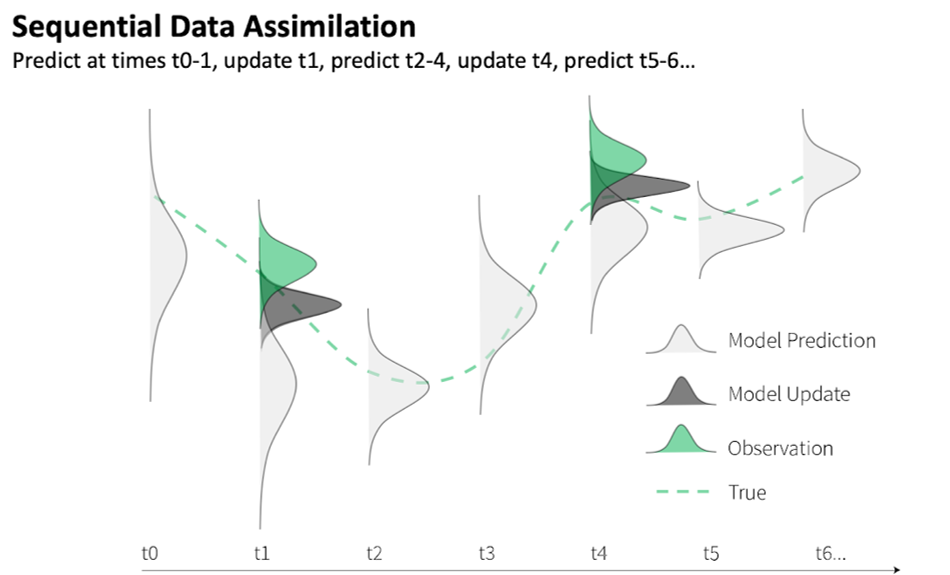
\includegraphics{images/Fig2_StatsMethodsUncertaintyTaskView.png}
\caption{Figure 2. In a sequential data assimilation framework, estimates of model states (and optionally parameters) are updated as new observations are assimilated into the model. The updated states take into account state observations and modeled state estimates as well as the relative confidence in each (shown as distributions). The updated states are then used as initial conditions for the model to make predictions at the next time step (t+1) using the model's equations. Figure from Ellen Bechtel and Jake Zwart.}
\end{figure}

For a given time step, a data assimilation algorithm takes two things as inputs: a joint probability distribution of model predictions for all model variables, and distributions of observations of a subset of those model variables. The data assimilation algorithm then synthesizes this information from both the model and the data and produces as output a new joint posterior distribution of all model variables (taking into account covariance between model variables). This new joint posterior distribution is used as the new model initial condition to generate updated predictions into the future (Figure 2).

\hypertarget{data-assimilation-approaches}{%
\subsection{Data assimilation approaches}\label{data-assimilation-approaches}}

Different data assimilation approaches (Table 1) differ in their assumptions about the distributions of the model and data predictions. Below we highlight some of the most commonly used data assimilation approaches.

\begin{itemize}
\item
  The simplest approach is the \textbf{Kalman Filter (KF; \href{https://github.com/EcoForecast/EF_Activities/blob/master/Exercise_09_KalmanFilter.Rmd}{EFI/NEON tutorial})}, which assumes that both model predictions and data have Gaussian (normal) distributions and that the model is linear. This assumption gives the Kalman filter a simple (iterative) analytical solution. Because of its computational efficiency and conceptual simplicity, implementations of the Kalman filter abound.

  \begin{itemize}
  \tightlist
  \item
    If you are using a model ensemble to estimate model uncertainty, the \textbf{ensemble Kalman filter (EnKF)} first fits a multivariate normal distribution (i.e., calculates the sample mean and covariance of the ensemble) and then proceeds as the normal Kalman filter.
  \item
    For highly computationally demanding models, where one is limited in the size of ensemble that can be used, the \textbf{unscented Kalman Filter (uKF)} uses the complex ``unscented transform'' to sample ensemble members systematically (rather than the random sampling in EnKF) and analytically back-transform the ensemble predictions to estimate the mean vector and covariance matrix (rather than the simple sample mean and covariance in EnKF).
  \end{itemize}
\item
  The linear model assumption of the Kalman filter can be relaxed by solving for the linear tangent approximation of model, much as one would do in initial two terms of a Taylor Series; this class of methods is called the \textbf{extended Kalman filter (eKF)}. Similar adjoint approaches are employed in variational data assimilation approaches (e.g.~4DVar).
\item
  The most general, completely distribution-agnostic data assimilation approach is the \textbf{particle filter (\href{https://github.com/EcoForecast/EF_Activities/blob/master/Exercise_10_ParticleFilter.Rmd}{EFI/NEON tutorial link})}, which simply resamples your model ensemble members weighted according to their likelihood relative to the observations. This approach is conceptually simple and typically easy to implement, but requires very large model ensembles and a variety of resampling methods to avoid rapid loss of effective sample size (prediction collapsing onto a small number of ensemble members that do not represent the true spread of the predictive distribution).
  Data assimilation is an active area of research, particularly in atmospheric science (not least because of its importance to numerical weather prediction), and new data assimilation approaches are constantly released. Some exciting recent developments (at least to the authors) include LaVEnDAR (\href{https://doi.org/10.5194/gmd-13-55-20200,\%20which\%20implements\%20an\%20ensemble\%20approach\%20to\%204DVar}{Pinnington et al.~2020}, the Tobit-Wishart ensemble filter (TWEnF, \href{https://www.biorxiv.org/content/10.1101/2020.05.05.079871v10}{Raiho et al.~2020}, which estimates the process error dynamically and accounts for zero-bound and zero-inflated data), and strongly coupled Earth System data assimilation techniques (\href{https://agupubs.onlinelibrary.wiley.com/doi/full/10.1029/2019MS001652}{Penny et al.~2019}), among others (Table 1).
\end{itemize}

In theory, data assimilation effectively and elegantly links uncertainties in parameters (see previous sections) and states. In practice, using data assimilation to track uncertainties in parameters and states simultaneously can be challenging (e.g., avoiding rapid convergence of all ensemble members to a single point) and often requires careful algorithm tuning. For example, Kalman Filter implementations sometimes artificially inflate the variance of the distributions to avoid convergence (e.g., filter inflation), but figuring out the right amount of inflation typically requires a lot of problem-specific trial and error (or methods that solve for the process error dynamically, e.g.~TWEnF).

\hypertarget{tools-for-data-assimilation}{%
\subsection{Tools for data assimilation}\label{tools-for-data-assimilation}}

Numerous tools exist for data assimilation , though a majority of these tools are targeted to large-scale models and big data and may be more complicated than needed for smaller ecological forecasting applications. Table 1 provides a sampling of the data assimilation tools available, but is by no means a comprehensive list.

\textbf{Table 1: Examples of data assimilation tools}

\begin{longtable}[]{@{}
  >{\raggedright\arraybackslash}p{(\columnwidth - 6\tabcolsep) * \real{0.11}}
  >{\raggedright\arraybackslash}p{(\columnwidth - 6\tabcolsep) * \real{0.29}}
  >{\raggedright\arraybackslash}p{(\columnwidth - 6\tabcolsep) * \real{0.22}}
  >{\raggedright\arraybackslash}p{(\columnwidth - 6\tabcolsep) * \real{0.38}}@{}}
\toprule
\textbf{Software} & \textbf{Software programming language} & \textbf{DA methods supported} & \textbf{Target application and model programming language supported} \\
\midrule
\endhead
\href{https://dart.ucar.edu/}{DART} & Fortran & KF, enKF & Large-scale models and big data in any language; originally created for atmospheric \& oceanic models \\
\href{https://r-nimble.org/}{Nimble} & R (with C++ backend) & Particle Filter, enKF & Small-scale models that can be implemented in R \\
\href{https://kingaa.github.io/pomp/}{pomp} & R & Particle Filter, enKF & Small-scale models that can be implemented in R \\
\href{https://www.mdpi.com/2311-5521/5/4/225}{PyDA} & Python & exKF, enKF, 3DVar, 4DVar & Small-scale models implemented in Python; originally created for researchers with little DA experience \\
\href{https://github.com/mschauer/Kalman.jl}{KalmanFilter.jl} & Julia & KF & Small-scale models that can be implemented in Julia \\
\href{https://github.com/ElOceanografo/StateSpace.jl}{StateSpace.jl} & Julia & KF, eKF, uKF, enKF & Small-scale models that can be implemented in Julia \\
\href{https://github.com/JuliaPOMDP/ParticleFilters.jl}{ParticleFilters.jl} & Julia & Particle Filter & Small-scale models that can be implemented in Julia \\
\href{http://www.met.reading.ac.uk/~darc/empire/index.php}{EMPIRE} & Python and Fortran & Particle Filter, enKF, 3DVar, 4DEnVar & Medium- to large-scale models that can be implemented in any language \\
\href{https://gmd.copernicus.org/preprints/gmd-2019-60/gmd-2019-60.pdf}{LaVEnDAR} & Python & 4DEnVar & Land surface models implemented in any language \\
\href{https://cran.r-project.org/web/packages/BayesianTools/index.html}{BayesianTools} & R & Particle Filter & Small- to Medium-scale models in any language \\
\href{https://www.openda.org/}{OpenDA} & C/C++, Java, Fortran & enKF, Steady State KF, Particle Filter, 3DVar, DudEnKF\textsuperscript{1} & Small- to large-scale models that can be implemented in any language \\
\bottomrule
\end{longtable}

\textsuperscript{1}DudEnKF - Doesn't Use Derivatives Ensemble Kalman Filter. See details \href{https://www.sciencedirect.com/science/article/pii/S0043135419311170}{here}.

  \bibliography{book.bib}

\end{document}
